\usetikzlibrary{patterns}

\usetikzlibrary{arrows}
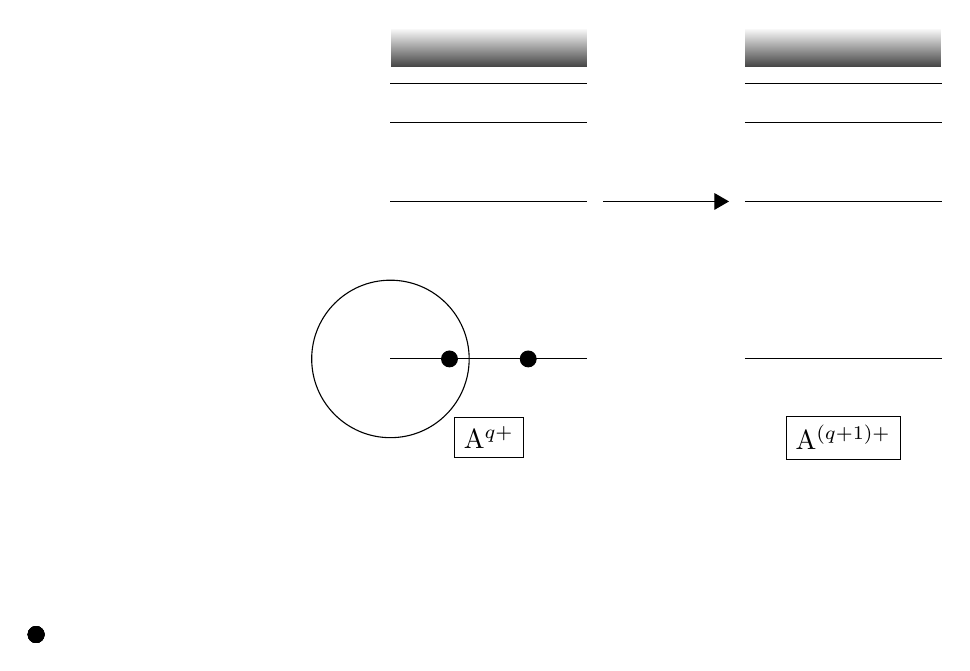
\begin{tikzpicture}
% Anker
\draw  (0,0) ellipse (1 and 1);
%

% Nr 1 Standard Darstellung ohne Elektronen
\draw (0,0) -- (2.5,0);
\draw (0,2) -- (2.5,2);
\draw (0,3) -- (2.5,3);
\draw (0,3.5) -- (2.5,3.5);
\shadedraw [draw=white,top color=lightgray!5,bottom color=darkgray] (0,3.7) rectangle (2.5,4.2);

% Nr 2 Standard Darstellung ohne Elektronen
\draw (4.5,0) -- (7,0);
\draw (4.5,2) -- (7,2);
\draw (4.5,3) -- (7,3);
\draw (4.5,3.5) -- (7,3.5);
\shadedraw [draw=white,top color=lightgray!5,bottom color=darkgray] (4.5,3.7) rectangle (7.0,4.2);

% Pfeile
\draw[-triangle 60] (2.7,2) -- (4.3,2);

% Elektronen
\filldraw  (0.75,0) ellipse (0.1 and 0.1);
\filldraw  (1.75,0) ellipse (0.1 and 0.1);
\filldraw  (-4.5,-3.5) ellipse (0.1 and 0.1);
\filldraw  (-4.5,-3.5) ellipse (0.1 and 0.1);

\filldraw  (-4.5,-3.5) ellipse (0.1 and 0.1);
\filldraw  (-4.5,-3.5) ellipse (0.1 and 0.1);
\filldraw  (-4.5,-3.5) ellipse (0.1 and 0.1);
\filldraw  (-4.5,-3.5) ellipse (0.1 and 0.1);
% Elektronenweg

% Beschriftung
\node[draw] at (1.25,-1) {A$^{q+}$};
\node[draw] at (5.75,-1) {A$^{(q+1)+}$};
\end{tikzpicture}